\section{Interrupts and Exceptions}

As already mentioned a few times in this thesis, MMIX does of course have a concept for \glslink{Interrupt}{interrupts} and \glslink{Exception}{exceptions} as well. It distinguishes four different kinds: \i{Forced trips}, \i{dynamic trips}, \i{forced traps} and \i{dynamic traps}.\footnote{Actually, the MMIX specification speaks of three kinds, because forced trips and dynamic trips are put together. \citep[pg. 28]{mmix-doc} But taking it as a whole, forced trips and dynamic trips conceptually differ in the same way as forced traps and dynamic traps do. Therefore, this thesis speaks of four kinds.} The first two are simply called \i{trips}, while the other two are called \i{traps}. The main difference is, that trips are handled by the user application, while traps are handled by the operating system.

\subsection{Triggering of Trips and Traps}

At first, the procedure of triggering a trip or trap is described. The forced trips and traps are requested explicitly by an instruction, whereas dynamic trips and traps are either raised because an exceptional condition occurred (synchronous) or an \glslink{Interrupt}{interrupt} occurred (asynchronous).

\subsubsection{Triggering Trips}

All trips make use of the special registers \sr{B}, \sr{W}, \sr{X}, \sr{Y} and \sr{Z}. Register \sr{B} is called \i{bootstrap register} and is used to save \dr{255}. The \i{where interrupted register} \sr{W} indicates the location the interruption occurred at, \i{execution register} \sr{X} holds the 4 instruction bytes and some other information. The registers \sr{Y} and \sr{Z} (\i{Y operand} and \i{Z operand}) are used to pass operands to the trip handler. \citep[pg. 28]{mmix-doc}

A forced trip can be triggered with the following instruction:
\instrtblfive
	{\mi{TRIP X,Y,Z}}
	{$\sr{X} \leftarrow 2^{63}~|$~\vmem{4}{@}}
	{$\sr{W} \leftarrow @ + 4$}
	{$\sr{Y} \leftarrow \dr{Y},\quad \sr{Z} \leftarrow \dr{Z}$}
	{$\sr{B} \leftarrow \dr{255},\quad \dr{255} \leftarrow \sr{J}$}
	{$@ \leftarrow 0$}
\noindent As the effect description shows, \mi{TRIP} puts various information into the special registers that can be used by the handler. The {\tt X} operand of the instruction is not used by the instruction itself, but since its bytes are put into \sr{X}, the handler may utilize it. Forced trips are always handled at address 0. \citep[pg. 28]{mmix-doc} The meaning of $2^{63}$ in \sr{X} and why \sr{J} is saved, will be explained when the handling of trips and traps is described.

Dynamic trips are raised for arithmetic \glslink{Exception}{exceptions}, which are controlled by \sr{A}. The only differences to forced trips are the location they are handled at and that \sr{Y} and \sr{Z} will be set to the decoded operands of the instruction that caused the \glslink{Exception}{AE}. Each arithmetic \glslink{Exception}{exception} has its own location:
$$\vbox{\halign{\hfil#:\quad &#\hfil\cr
	\haddr{10} & Integer divide check (D)\cr
	\haddr{20} & Integer overflow (V)\cr
	\haddr{30} & Float-to-fix overflow (W)\cr
	\haddr{40} & Invalid operation (I)\cr
	\haddr{50} & Floating overflow (O)\cr
	\haddr{60} & Floating underflow (U)\cr
	\haddr{70} & Floating division by zero (Z)\cr
	\haddr{80} & Floating inexact (X)\cr
}}$$
Forced and dynamic trips are triggered in user mode only, \ie they are ignored in privileged mode. \citep[pg. 28]{mmix-doc}

\subsubsection{Triggering Traps}

Similarly to trips, traps use the special registers \sr{BB}, \sr{WW}, \sr{XX}, \sr{YY} and \sr{ZZ}, with the same purposes as their trip correspondences. The reason for the separate registers is, that a trap may of course be triggered while a trip is handled. Additionally, register \sr{T} specifies the location at which forced traps are handled, whereas \sr{TT} specifies the location for dynamic traps. \citep[pg. 28,29]{mmix-doc}

MMIX uses the special \i{interrupt mask register} \sr{K} to control which dynamic traps are enabled. As soon as a bit in the special \i{\glslink{Interrupt}{interrupt} request register} \sr{Q} is 1 and the corresponding bit in \sr{K} is 1 as well, a dynamic trap is triggered. These registers have the following layout:
\begin{figure}[H]
	\centering
	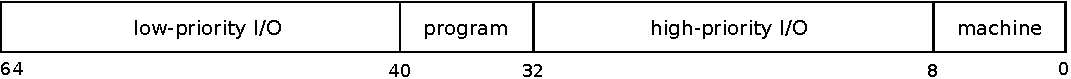
\includegraphics[width=\textwidth]{img/rKrQ-crop.pdf}
\end{figure}
\vspace{-20pt}
\noindent In general, the bits on the right have a higher priority than the bits on the left. Therefore, high-speed devices like network cards should get bits on the right, while slow devices like terminals should get bits on the left. But MMIX does not define the meanings of the I/O bits. Only the program (\glslink{Exception}{PEs}) and some of the machine bits (\glslink{Exception}{MEs}) are specified. The program bits are called {\tt rwxnkbsp} with the following meanings:
$$\vbox{\halign{{\tt #} bit: &#\hfil\cr
r	&	instruction tries to load from a page without read permission;\cr
w	&	instruction tries to store to a page without write permission;\cr
x	&	instruction appears in a page without execute permission;\cr
n	&	instruction refers to a privileged (negative) address;\cr
k	&	instruction is privileged, for use by the kernel only;\cr
b	&	instruction breaks the rules of\/ MMIX;\cr
s	&	instruction violates security (see below);\cr
p	&	instruction comes from a privileged address.\cr}}$$
The four specified machine bits from right to left stand for power failure, memory parity error, nonexistent memory and rebooting. MMIX defines, that the program bits have to be set in \sr{K} when executing in user mode (otherwise a security \glslink{Exception}{PE} is raised) and that program bit {\tt p} has to be zero in \sr{K} when executing in privileged mode (otherwise a privileged \glslink{Exception}{PE} is raised). \citep[pg. 29]{mmix-doc}

Analogous to the forced trip, the forced trap instruction is defined as:
\instrtblsix
	{\mi{TRAP X,Y,Z}}
	{$\sr{XX} \leftarrow 2^{63}~|$~\vmem{4}{@}}
	{$\sr{WW} \leftarrow @ + 4$}
	{$\sr{YY} \leftarrow \dr{Y},\quad \sr{ZZ} \leftarrow \dr{Z}$}
	{$\sr{BB} \leftarrow \dr{255},\quad \dr{255} \leftarrow \sr{J}$}
	{$\sr{K} \leftarrow 0$}
	{$@ \leftarrow \sr{T}$}
\noindent That means, besides the different handler location and the different set of special registers, \mi{TRIP} and \mi{TRAP} are equivalent, except that \mi{TRAP} clears \sr{K}. This way, dynamic traps are disabled. \citep[pg. 28]{mmix-doc} The operating system may even use instructions in a way that would raise a \glslink{Exception}{PE}, if the corresponding bit in \sr{K} were set. Because MMIX defines that "an instruction that traps with bits {\tt x}, {\tt k} or {\tt b} does nothing; a load instruction that traps with {\tt r} or {\tt n} loads zero; a store instruction that traps with any of {\tt rwxnkbsp} stores nothing" \citep[pg. 29]{mmix-doc}. The meaning of the operands {\tt X}, {\tt Y} and {\tt Z} can be defined by the operating system for any purpose. But two settings are predefined by MMIX:
\begin{enumerate}
	\item ${\tt XYZ} = 0$ should terminate the user process and
	\item ${\tt XYZ} = 1$ should offer a default action for a trip, for which the user program has not provided a handler (thus, instead of handling the trip, it can do a \mi{TRAP 0,0,1}).
\end{enumerate}

Analogous to forced and dynamic trips, the differences between forced and dynamic traps are, that for dynamic traps, the operands in \sr{YY} and \sr{ZZ} correspond to the operands of the interrupted instruction and the handler location is different. Additionally, MMIX defines that if "the interrupted instruction contributed 1s to any of the {\tt rwxnkbsp} bits of \sr{Q}, the corresponding bits are set to 1 also in \sr{XX}" \citep[pg. 29]{mmix-doc}. More precisely, these bits occur in the first byte of the upper tetra of \sr{XX}.

\subsection{Handling of Trips and Traps}

After having described the mechanisms of triggering trips and traps, it should be explained how they can be handled. This section starts with the instruction that resumes an interrupted computation, followed by the handling of trips and traps.

\subsubsection{Resuming}

Of course, MMIX has to be able to resume the ordinary execution after a trip or trap has been handled. To do so, it provides a quite sophisticated instruction that can be used for various purposes.

\instrtbleight
	{\mi{RESUME Z}}
	{if ${\tt Z} = 1$:}
	{$\quad \sr{K} \leftarrow \dr{255},\quad \dr{255} \leftarrow \sr{BB}$}
	{$@ \leftarrow \sr{W}|\sr{WW}$}
	{ropcode$~\leftarrow (\sr{X}|\sr{XX}) \gg 56$}
	{if ropcode$~= 0$: repeat(\sr{X}|\sr{XX})}
	{if ropcode$~= 1$: continue(\sr{X}|\sr{XX})}
	{if ropcode$~= 2$: set(\sr{X}|\sr{XX})}
	{if ${\tt Z} = 1~$and ropcode$~= 3$: trans(\sr{X}|\sr{XX})}
\noindent The instruction \mi{RESUME} comes in two versions: \mi{RESUME 0} resumes the computation after a trip, while \mi{RESUME 1} resumes it after a trap. Thus, \mi{RESUME 0} uses \sr{W} and \sr{X}, while \mi{RESUME 1} uses \sr{WW} and \sr{XX}. That does also mean, that the latter is prohibited in user mode. The default behaviour of \mi{RESUME}, when the so called \i{ropcode} is \haddr{80} (see \mi{TRIP} and \mi{TRAP}), is quite simple. The trip-version continues the execution at \sr{W}, while the trap-version sets \sr{K} and \dr{255} first and continues at \sr{WW} afterwards. But as the effect description shows, there are four other defined values of ropcode, which are more complicated. The four sketchy described actions have the following meaning:
\begin{itemize}
	\item repeat(\sr{X}|\sr{XX}):\\
	MMIX interprets the lower four bytes of \sr{X}|\sr{XX} as an instruction and executes it. This is allowed for all instructions except \mi{RESUME} itself.
	\item continue(\sr{X}|\sr{XX}):\\
	Continue is similar to repeat. It does also interpret the lower four bytes of \sr{X}|\sr{XX} as an instruction. But it does not use the operands provided in the instruction, but takes \sr{Y}|\sr{YY} and \sr{Z}|\sr{ZZ} instead. It is allowed for all "Set \dr{X} to the result of \dr{Y} OP \udrim{Z}" and "Set \dr{X} to the result of OP \udrim{Z}" instructions and for \mi{TRAP} as well. Some implementations of MMIX may also allow \mi{SYNCD} and \mi{SYNCID}. Another restriction is, that the instruction can not increase \sr{L}, \ie the {\tt X} operand of the instruction has to be less than \sr{L}.
	\item set(\sr{X}|\sr{XX}):\\
	This ropcode tells MMIX to set the register, denoted by the third least significant byte of \sr{X}|\sr{XX}, to \sr{Z}|\sr{ZZ}. Additionally, the third most significant byte is used to raise \glslink{Exception}{AEs}. Again, \sr{L} can not be increased.
	\item trans(\sr{X}|\sr{XX}):\\
	Last but not least, this ropcode can be used to put a translation into the translation cache. It uses \sr{YY} as the virtual address and \sr{ZZ} as the PTE and puts it into a TC. If the opcode of the instruction in the lower half of \sr{XX} is \mi{SWYM} (\i{sympathize with your machinery}; the NOP instruction of MMIX, that does nothing), the translation will be put into the instruction TC, otherwise in the data TC. Additionally, if this opcode is not \mi{SWYM}, the action repeat(\sr{XX}) will be performed.
\end{itemize}
All these actions behave as if they appeared as an instruction at location $\sr{W}|\sr{WW}-4$, \ie as if they have been inserted into the instruction stream at that position. \citep[pg. 30]{mmix-doc} It will be described shortly for what reasons the different actions, depending on ropcode, are offered.

\subsubsection{Handling Trips}

As said in the last section, all different kinds of trips have their own handler location, which are 16 bytes away from each other. That means, each handler has 4 instructions available to do what ever is necessary. For example, it could do something like:
\begin{center}
	\lstinline`PUSHJ $255,Handler; PUT rJ,$255; GET $255,rB; RESUME 0`
\end{center}
This way, the actual handler is called, saving all local registers on the stack. Before resuming, \sr{J} and \dr{255} have to be restored, because -- as described previously -- \mi{RESUME} will not do that. \citep[pg. 28]{mmix-doc}

Another way is to let the operating system perform the default actions for a trip by:
\begin{center}
	\lstinline`TRAP 0,0,1; GET $255,rB; RESUME 0`
\end{center}
In this case, no subroutine is called and thus, \sr{J} has not to be restored. \citep[pg. 28]{mmix-doc} Additionally, the reason why \mi{RESUME} does not restore the values saved by \mi{TRIP}, is that MMIX pursues the goal to perform only the minimum set of actions that are required.

When handling a dynamic trip, the operands of the instruction that caused the \glslink{Exception}{AE} are put into \sr{Y} and \sr{Z}. For example, if \mi{DIV \$0,\$1,0} is executed, MMIX will raise a division by zero \glslink{Exception}{AE} and set \sr{Y} to \$1 and \sr{Z} to 0. The handler could simply recognize that an \glslink{Exception}{AE} occurred. But it could also replace \sr{Y} and \sr{Z} with something else and change the ropcode in \sr{X} from \haddr{80} to \haddr{01} (continue). This way, the instruction would be repeated with operands \sr{Y} and \sr{Z}. Another way would be to set the ropcode to \haddr{02}, which would set \dr{X} to the value specified in \sr{Z}. \citep[pg. 28]{mmix-doc}

\subsubsection{Handling Traps}

Similarly to dynamic trips, dynamic traps that are triggered because of a \glslink{Exception}{PE}, save the operands of the instruction that caused it in \sr{YY} and \sr{ZZ}. MMIX does not define the meaning of these registers for all instructions. But it is defined that all "Set \dr{X} to the result of \dr{Y} OP \udrim{Z}" instructions put \dr{Y} in \sr{YY} and \udrim{Z} into \dr{Z}. Additionally, load instructions put the virtual address into \sr{YY}\footnote{Unfortunatly, the specification does not mention that explicitly for loads. But MMIX-PIPE does behave as explained and it would make no sense to do it for store instructions, but not for load instructions. After all, both may trigger a protection fault, for which the operating system has to know the virtual address. Having to calculate it from the {\tt Y} and {\tt Z} operand of the instruction for loads and simply read it from \sr{YY} for stores, would be very strange.}, while store instructions do additionally put the octa to be stored (including unchanged bytes for cases like \mi{STB}) into \sr{ZZ}. \citep[pg. 27]{mmix-doc}

Additionally it is noteworthy, that the OS has not many choices when considering \glslink{Exception}{PE} handling. Because the only \glslink{Exception}{PEs}, which are well defined, are the protection faults. For all others, \ie when refering to a negative address, using a privileged instruction, breaking the rules of MMIX, violating security or jumping to a privileged address, the MMIX specification does not define the values of \sr{WW} and \sr{XX}. Thus, the operating system is unable to resume the computation of the user program in a reliable way. But of course, these \glslink{Exception}{PEs} indicate a malicious or faulty user program anyway, so that the best option is a kill (and perhaps providing feedback to the user in form of a log entry or similar).

MMIX does also allow cheaper implementations of it, that let the software realize some instructions. In this case, these instructions cause a forced trap. For example, expensive operations like \mi{DIV} or \mi{FREM} could be implemented in software by checking the opcode in \sr{XX} when handling a forced trap. If it is one of these instructions, the result will be computed, put into \sr{ZZ} and the ropcode will be set to \haddr{02}. A subsequent \mi{RESUME 1} will place \sr{ZZ} into the desired register. As already said, even arithmetic \glslink{Exception}{exceptions} could be raised by specifying them in the third most significant byte of \sr{XX}. \citep[pg. 28]{mmix-doc}

A similar feature is, that address translation can be done in software. This can be requested by setting field $f$ of \sr{V} to 1, but some implementations of MMIX might even require that. As soon as a translation is necessary, \ie it is not already in the corresponding TC, a forced trap with ropcode \haddr{03} is triggered. The virtual address will be available in \sr{YY}. When the translation is done, the handler should put the physical address into \sr{ZZ}. A subsequent \mi{RESUME 1} will put this translation into the TC and repeat the instruction, which will succeed this time. It should be noted, that if an instruction fetch fails, MMIX will put the instruction \mi{SWYM} into \sr{XX}. This way, the translation will be put into the instruction TC and the fetch will be repeated when \mi{RESUME 1} is executed. \citep[pg. 28]{mmix-doc}

\subsection{Interruptibility}
\label{sec:mmix-interruptibility}

Because of the complexity of some instructions (like \mi{SAVE}, \mi{POP}, \mi{DIV}, \mi{FREM} and so on), MMIX allows them to be interruptible. The specification words it as:
\begin{quote}
Non-catastrophic \glslink{Interrupt}{interrupts} in MMIX are always precise, in the sense that all legal instructions before a certain point have effectively been executed, and no instructions after that point have yet been executed. The current instruction, which may or may not have been completed at the time of \glslink{Interrupt}{interrupt} and which may or may not need to be resumed after the \glslink{Interrupt}{interrupt} has been serviced, is put into the special execution register \sr{X}, and its operands (if any) are placed in special registers \sr{Y} and \sr{Z}.\footnote{Actually, \sr{XX}, \sr{YY} and \sr{ZZ} are meant (which were introduced later in the specification), because the other ones are only used for trips, which are either explicitly requested or raised for \glslink{Exception}{AEs}. Thus, they do not occur at arbitrary points of time during a computation, as \glslink{Interrupt}{interrupts} from I/O devices may.} \citep[pg. 27]{mmix-doc}
\end{quote}
That means, if an \glslink{Interrupt}{interrupt} occurs while executing an instruction, a particular MMIX implementation may wait briefly until an interruption is possible and then put the state of computation of the current instruction into \sr{XX}, \sr{YY} and \sr{ZZ}. In this case, the meaning of the registers is completely implementation dependent. For example, \mi{FREM \$X,\$Y,\$Z} may set \sr{YY} and \sr{ZZ}, such that $\sr{YY} \bmod \sr{ZZ} = \dr{Y} \bmod \dr{Z}$, but the actual values of \sr{YY} and \sr{ZZ} may be different than \dr{Y} and \dr{Z}. \citep[pg. 27 and 29]{mmix-doc} If MMIX sets ropcode to \haddr{01} (continue), the operating system will not be required to care about that, because a \mi{RESUME 1} will simply execute that instruction again with \sr{YY} and \sr{ZZ}, which will lead to the same result.

It should also be mentioned, that \sr{XX} might not hold the instruction found at address $\sr{WW}-4$. Not only because of jumps, but also because MMIX might put an instruction into \sr{XX}, that has been inserted internally. For example, if \mi{ADD \$X,\$Y,\$Z} is executed with ${\tt X} \ge \sr{L}$, the hardware may insert an instruction to increase \sr{L} first.

